\section{用.csv文件绘制table}
这节做的不理想,经常报错。略过。
\section{用.csv文 件简单绘图}
\begin{figure}[h!]
  \begin{center}
    \begin{tikzpicture}
      \begin{axis}[
          width=\linewidth, 
          grid=major, % 显示网格
          grid style={dashed,gray!30}, % Set the style
          xlabel=X Axis $U$, % Set the labels
          ylabel=Y Axis $I$,
          x unit=\si{\volt}, % 设置单位
          y unit=\si{\ampere},
          legend style={at={(0.5,-0.2)},anchor=north}, % 在图下显示图例
          x tick label style={rotate=90,anchor=east} % 显示横坐标
        ]
        \addplot 
        % the .csv file (on top), 注意.csv文件中前两行的名字与x,y的名字相一致
        table[x=column 1,y=column 2,col sep=comma] {second/table.csv}; 
        \legend{Plot}
      \end{axis}
    \end{tikzpicture}
    \caption{My first autogenerated plot.}
  \end{center}
\end{figure}
\section{tikz绘制矢量图}
mindmaps是思维导图的意思,flowchart流程图。
\begin{figure}[h!]
	\begin{center}
		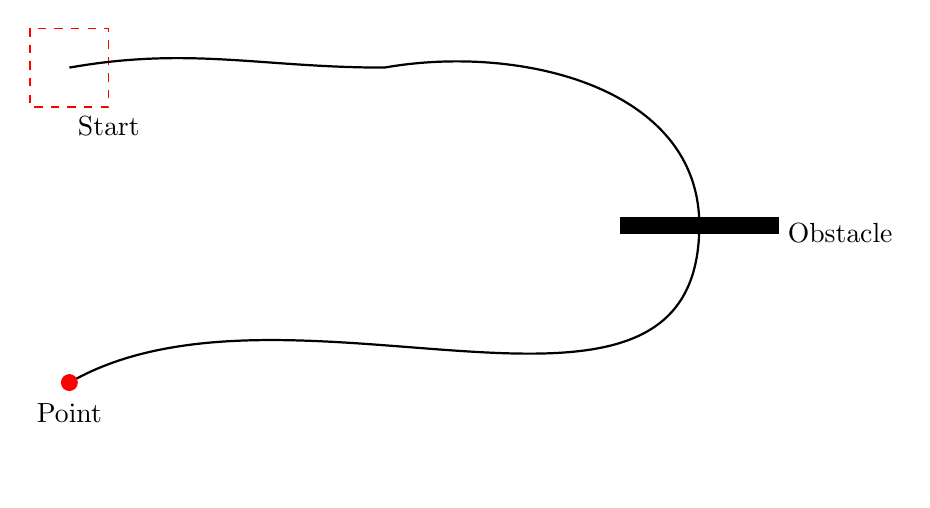
\begin{tikzpicture}
		     % 画矩形是确定对角线两点的坐标,start是字体
			\draw[red,dashed](-2.5,2.5) rectangle (-1.5,1.5)  node[black,below]{Start};
			\draw[thick](-2,2) 
			%设置入和出的角度,出是(-2,2)的出角度,入是进入(2,2)的角度,角度是按照极坐标系来算
			to [out=10,in=180] (2,2)
			to[out=10,in=90] (6,0)
			to[out=-90,in=30](-2,-2);
			\draw[fill](5,0.1) rectangle(7,-0.1) node[black,right]{Obstacle};
			\draw[red,fill] (-2,-2)  circle[radius=0.1] node[black,below=4]{Point};
		\end{tikzpicture}
	\end{center}
\end{figure}
\section{高亮源代码}
用listings包可以解决源代码高亮。
% \renewcommand\lstlistingname{Quelltext}
% 设置源代码区域显示格式
注意必须设置源代码中的注释和关键字的颜色,否则输出只有黑色和白色。
源代码包含在listings环境中。直接在LaTeX中写代码,遇到注释$\backslash\backslash$和$\ast$需要转义。
\lstset{
	language=Java,
	basicstyle=\small\sffamily,
	numbers=left,
	numberstyle=\tiny,
	frame=tb,
	tabsize=4,
	columns=fixed,
	showstringspaces=false, %在字符串的空格中显示一个下划线_
	showtabs=false, %在tab显示一个下划线_
	keepspaces=true, % keeps spaces in text, useful for keeping indentation of code (possibly needs columns=flexible), 暂且不知道什么作用
	commentstyle=\color{green},
	keywordstyle=\color{blue}
}
\begin{lstlisting}
public class Hello{
	public static void main(String[]args){
			System.out.println(''hello  world!'');
	}
}
\end{lstlisting}
再写一段代码, 也可以直接输入源代码的文件,而避免在LaTeX文档中输入代码。也不用注意代码中触及到LaTeX的关键字。
\lstinputlisting{second/hello.java}
\section{circuitikz绘制电路图}
\subsection{绘制基本电路图}
\begin{figure}[h!]
	\begin{center}
		\begin{circuitikz}
			\draw(0,0)
			to[V=$U_q$] (0,2)  % 电压源
			to[short] (2,2)          % 导线
			to[R=$R_1$] (2,0)  % 电阻
			to[short] (0,0) ;
			\draw (2,2)
			to[short] (4,2)
			to[L=$L_1$] (4,0)
			to[short] (2,0);
			\draw (4,2)
			to[short] (6,2)
			to[C=$C_1$] (6,0)
			to[short] (4,0);
		\end{circuitikz}
		\caption{My first circuit}
	\end{center}
\end{figure}

\subsection{circuit的高级使用}
\begin{figure}[h!]
	\begin{center}
		\begin{circuitikz}
			\draw (-1,0) to[short ,o-o] (1,0); % 两端用空心圆点连接
			\draw (0,0) to [short] node[ground] {GND} (0,-1);  %画出接地的标识
			\draw (-1,1) to[short ,*-] (1,1);   %两端用实心圆点和无圆点连接
		\end{circuitikz}
	\end{center}
\end{figure}

\subsection{画电路流向}
方向是通过circuitikz默认决定的,但是我们可以覆写。
\begin{figure}[h!]
	\begin{center}
		\begin{circuitikz}
			\draw (0,0) to[R,i^<=$i_1$] (2,0); % <是指明电流流向,_是让i1文字标识在下面,^是标注在上面
			\draw (0,-2) to [R,v>=$u_1$] (2,-2); %指明电压方向
			\draw (0,-4) to [R,l=$R_1$] (2,-4); %画一个电阻, l标识label标签
		\end{circuitikz}
	\end{center}
\end{figure}
\subsection{三极管}
\begin{figure}[h!]
	\begin{center}
		\begin{circuitikz}
		\draw (0,0) node[npn](npn1) {}
		(npn1.base) node[anchor=east] {B}
		(npn1.collector) node[anchor=south,xshift=0.5cm] {C}
		(npn1.emitter) node[anchor=north] {E};
		\draw (npn1.collector) to [R] ++(0,2); % (0,2)标识C端口的水平垂直位移
		\end{circuitikz}
	\end{center}
\end{figure}
\section{超链接hyperlink}
在MikTeX中编译包含hycolor.sty的时候,总是显示找不到hycolor.sty,在ctan中下载了hycolor.dtx之后, 执行以下命令
\begin{lstlisting}
$: tex hycolor.dtx
\end{lstlisting}
解压出hycolor.sty,放在.tex同一目录下,一起编译就可以。
\subsection{超链接}
超链接的蓝色的框,只在PDF显示中出现,在打印中不会出现。
这是个超链接,\href{http://www.baidu.com}{百度一下,你就知道}。
\subsection{URL}
嵌入一个简单的URL,\url{https://www.baidu.com}
\subsection{邮件地址}
邮件地址是: \href{george:usa@163.com}{usa@163.com}
\section{列表}
\subsection{无序列表}
\begin{itemize}
	\item One
	\item Two
	\item Three
\end{itemize}
\subsection{有序列表}
\begin{enumerate}
	\item One
	\item Two
	\item Three
\end{enumerate}
\subsection{嵌套列表}
\begin{enumerate}
	\item One
	\begin{enumerate}
		\item o
		\item n
		\item e
	\end{enumerate}
	\item two
	\item three
\end{enumerate}
\subsection{无序列表前的装饰}
可以修改无序列表前的装饰,而不是默认的黑点
\begin{itemize}
	\item[$-$] Dash
	\item[$\ast$] Asterisk
\end{itemize}
另外一种修改的方法, 统一指定前缀装饰
\begin{itemize}[label=$\ast$]
	\item one
	\item two
	\item three
\end{itemize}
\subsection{修改有序列表的前缀}
加载enumitem包,可以修改为字母,数字,罗马数字等。
\subsubsection{罗马数字}
\begin{enumerate}[label=(\roman*)]
	\item one
	\item two
	\item three
\end{enumerate}
\subsubsection{阿拉伯数字}
\begin{enumerate}[label=(\arabic*)]
	\item one
	\item two
	\item three
\end{enumerate}
\subsubsection{字母}
\begin{enumerate}[label=(\alph*)]
	\item one
	\item two
	\item three
\end{enumerate}